\chapter{The High Granularity Calorimeter}
\label{chap:hgcal}

\section{The High Luminosity LHC}

Run~2 of the LHC is now complete, with over $\SI{150}{\fbinv}$ of data collected at $\sqrt{s}\,=\,\SI{13}{TeV}$. %original target was 150 Run 1 plus Run 2
This was achieved partly because the machine was eventually operated at twice its nominal instantaneous luminosity, resulting in values of at $\SI{2e34}{\lumi}$ during 2018.
The second long shutdown (LS2) commenced following the completion of Run~2 and will last until 2021.
During this time various improvements to the LHC will be made, including a substantial upgrade to the injection system.
The machine will also be readied for operation at the increased energy of $\SI{7}{TeV}$ per beam.
However these upgrades will not substantially affect the conditions experienced by the LHC experiments; 
the peak instantaneous luminosity is not envisaged to increase beyond $\SI{2e34}{\lumi}$.
As such no major changes are required to the CMS detector during LS2, although various improvements are planned: 
these include upgrades to the muon system and HCAL barrel.
Therefore the expectation for Run~3, commencing in 2021 with two years of high-availability data-taking in 2022 and 2023, 
is that a further $\SI{150}{\fbinv}$ of data at will be accumulated. 
%See here for details of LS2 and Run 3: https://indico.cern.ch/event/773482/contributions/3213751/attachments/1763994/2863045/LHC-Run2.CMS.Dec18.JW.pdf

Beyond Run~3, the usefulness of running the LHC with its current parameters decreases.
In order to reduce the statistical error on physics measurements by a factor of two, high-availability operation for more than ten years would be required.
Therefore a major upgrade to the LHC is planned, referred to as the Phase~2 upgrade, to maximise its physics reach.
%insert info about what is actually being upgraded here? %TODO learn a bit about the things below 
%The technological innovations facilitating the upgrade include $\SI{12}{T}$ superconducting magnets, compact and precise superconducting cavities, and new beam collimation technology.
The resulting High~Luminosity~LHC (HL-LHC) \cite{HLLHC} will have an nominal levelled instantaneous luminosity of $\SI{5e34}{\lumi}$, 
permitting a total of $\SI{3000}{\fbinv}$ of data to be collected by the mid-2030s.
The current planned schedule of the future running of the LHC and HL-LHC is summarised in Figure~\ref{fig:hgcal_LHCschedule}.

The corresponding mean pileup is per bunch crossing is 140; however an additional 50\% beyond the nominal value is allowed for in the HL-LHC design, 
which would result in mean pileup values of up to 200.
This constitutes a major change, and the environment will be significantly harsher than with the current LHC conditions, 
posing serious challenges to the detectors in terms of radiation tolerance and reconstruction in high pileup.
Therefore in order to maintain or improve upon the excellent performance exhibited in Run~2, a suite of upgrades to the CMS detector are planned.
The key aspects of the CMS Phase~2 upgrade can be summarised as \cite{UpgradeTP}:
\begin{itemize}
  \item{\textbf{Tracker:}
  the tracker will suffer significant radiation damage and must be entirely replaced for Phase~2.
  The upgraded tracker will have an granularity, %factor of 4
  increased coverage in the forward region, %up to eta=4
  and be much lighter, resulting in a reduced material budget.
  Furthermore, the design will allow track information to be included in the L1 trigger decision.}
  %enabling powerful background rejection at the earliest event selection step
  \item{\textbf{Endcap calorimeters:}
  the calorimeter endcaps (both ECAL and HCAL) will also be radiation-damaged by the end of Run~3, and will therefore be replaced.
  The replacement design, known as the high granularity calorimeter (HGCAL), will have both electromagnetic and hadronic sections.
  Fine segmentation in each of the longitudnal and transverse directions will facilitate precise measurements of showers in three-dimensions.}
  \item{\textbf{Muon endcaps:}
  the CSC forward muon system will be enhanced with additional stations.
  This will increase the forward coverage and maintain muon acceptance at the L1 trigger.}
  %because new bits provide redundancy (only 1.5 to 2.4 doesn't have redundancy in muon system atm) and timing resolution.
  \item{\textbf{Trigger and data acquisition:}
  due to the tracker upgrade, the latency of the L1 trigger at Phase~2 is increased to \SI{12.5}{\micro\second}.
  Combined with upgrades to the front-end electronics of various subdetectors, %barrel calorimeter; the CSCs of the inner rings, and the DT readout.
  this enables an increase of the L1 trigger acceptance rate to \SI{500}{\kilo\hertz}.
  Consequently the data acquisition system must also be upgraded to handle the increase in event rate, event size, and the complexity of high PU reconstruction.}
\end{itemize}
The remainder of this chapter is describes the HGCAL in further detail.

%FIXME this figure is out of date
\begin{figure}[h!]
  \centering
  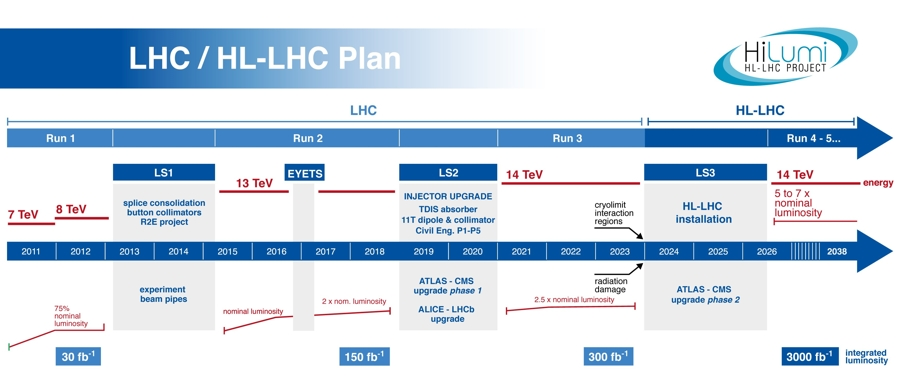
\includegraphics[width=\textwidth]{Figures/HGCAL/LHCschedule.jpg}
  \caption[Planned LHC and HL-LHC schedule]
  {The planned schedule for the operation of the LHC and its high-luminosity upgrade.
  (Need to find a more up-to-date version of this figure).}
  \label{fig:hgcal_LHCschedule}
\end{figure}


\section{The HGCAL}

\subsection{Requirements}

The primary challenge which drives the design of the HGCAL is the need to sustain physics performance in the extremely high pileup conditions foreseen at the HL-LHC.
Simulations indicate that the HGCAL will be required to withstand up to 2MGy of total radiation dose, together with a maximum fluence of around $\SI{10e16}{\textrm{n}_{\textrm{eq}}/\textrm{cm}^2}.$
%The distribution of the radiation dose throughout the detector is shown in Figure \ref{fig:RadiationDose}. 
Studies performed in recent years have shown that silicon sensors and the associated electronics retain acceptable performance after exposure to this level of radiation, 
and have hence been chosen as the most reliable active material for the majority of the calorimeter. 
The remaining parts of the detector in lower-radiation regions will instead use cheaper plastic scintillator tiles with silicon photomultipliers (SiPMs). 

To maintain performance throughout the operation of the HL-LHC it is necessary to inter-calibrate cells to the level of a few percent. 
This can be achieved with a sufficiently high signal-to-noise ratio (S/N) for minimum-ionising particles (MIPs), after $\SI{3000}{\fbinv}$.
Consequently small silicon cells with low capacitance are required, resulting in high lateral granularity. 
Fine lateral granularity also has many benefits for physics performance, including the ability to separate nearby showers, 
identify narrow jets such as those originating from vector boson fusion (VBF), and minimise the amount of pileup entering energy measurements. 
To take advantage of this fine segmentation the calorimeter is required to be dense, thereby preserving the compactness of showers in the transverse direction.
Similarly, fine longitudinal granularity facilitates precise energy measurements, as well as enabling discrimination between different types of shower using the depth profile.
These features are particularly important within the CMS particle flow reconstruction paradigm \cite{ParticleFlow}. 
A detector producing three-dimensional images of showers would provide powerful separation of electromagnetic, charged hadronic and neutral hadronic components, 
facilitating more precise energy measurements, particularly of jets. 

In addition, the HGCAL should be able to perform precise timing measurements enabling excellent pileup rejection, and provide an input to the level one trigger decision. 
The proposed design specification that captures all of these desired features is described in the following section. 

\subsection{Design}

\begin{figure}[h!]
\begin{centering}
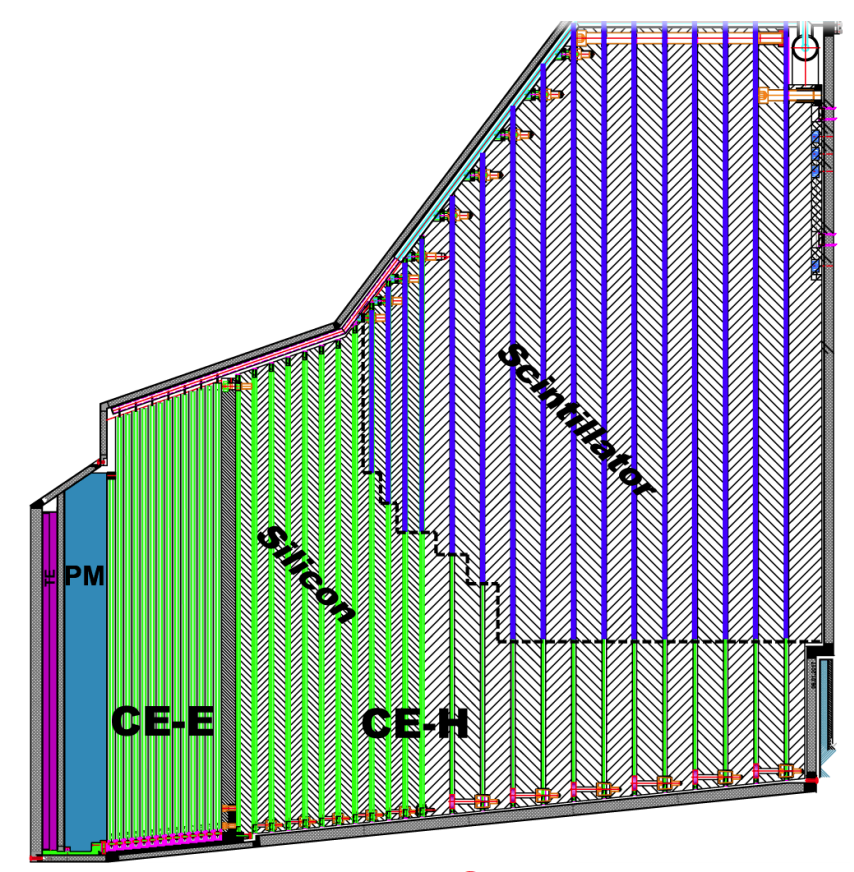
\includegraphics[width=0.7\textwidth]{Figures/HGCAL/TheHGCAL.png}
\caption{A schematic of the HGCAL. Adapted from \cite{HGCAL}.}
\label{fig:TheHGCAL}
\end{centering}
\end{figure}

An overview of the HGCAL design is presented in Figure \ref{fig:TheHGCAL}.
The HGCAL is composed of an electromagnetic and a hadronic section, called the CE-E and CE-H respectively, covering the pseudorapidity range $1.5 < |\eta| < 3.0$.
The CE-E comprises 28 layers with hexagonal silicon sensors as the active element. 
The total depth, including the neutron moderator layer at the front, is \SI{34}{cm}, which corresponds to approximately \SI{26}{$X_0$} and \SI{1.7}{$\lambda$}. 
Three different thicknesses of silicon sensors are used, with thickness decreasing as a function of fluence. 
Absorbers are made of WCu and Cu plates are used for cooling. 
All layers of the CE-E are used for energy measurements, but alternate layers give inputs to the L1 trigger primitive formation. 

The CE-H is formed of 12 layers with \SI{35}{mm} thick stainless steel (SS) absorber and another 12 with \SI{68}{mm} thick SS absorber, contributing an additional \SI{9}{$\lambda$} in depth. 
The active medium in the CE-H varies as a function of depth and radius, and is determined by the radiation level. 
In regions of sufficiently low fluence (those which are furthest back and furthest from the beam-pipe), plastic scintillator tiles are used with SiPM readout. 
The exact threshold between the scintillator and silicon is determined by the S/N required to measure the MIP response, which is decreased by exposure to radiation. 
Further detail on the design specifications of the HGCAL can be found in \cite{HGCAL}. 

\subsection{Reconstruction}

\begin{figure}[h!]
\begin{centering}
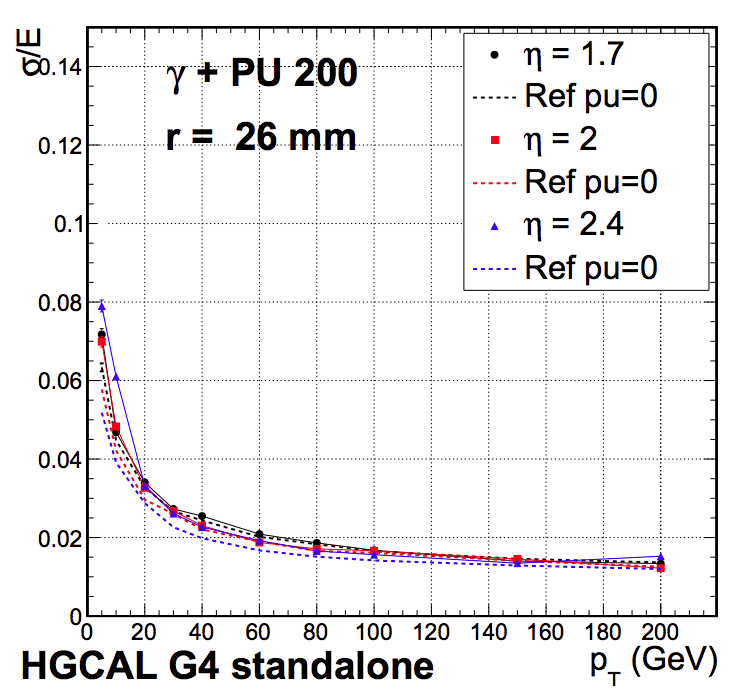
\includegraphics[width=0.45\textwidth]{Figures/HGCAL/SinglePhotonReso.png}
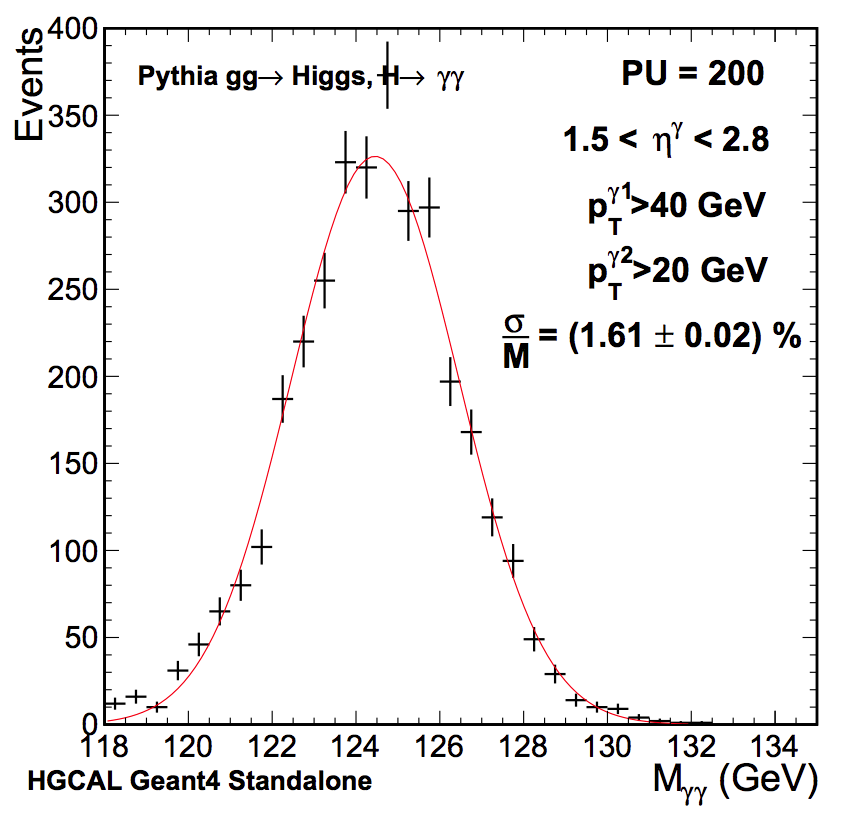
\includegraphics[width=0.45\textwidth]{Figures/HGCAL/HggReso.png}
\caption{
Left: the intrinsic energy resolution for single photons in PU200. The energy is estimated by summing all deposits within a \SI{26}{mm} radius of the generated particle axis. 
Right: the intrinsic diphoton mass resolution of the HGCAL in simulated \Hgg events where both photons are within the fiducial region of the HGCAL. Both taken from \cite{HGCAL}.}
\label{fig:PhotonReso}
\end{centering}
\end{figure}

\begin{figure}[h!]
\begin{centering}
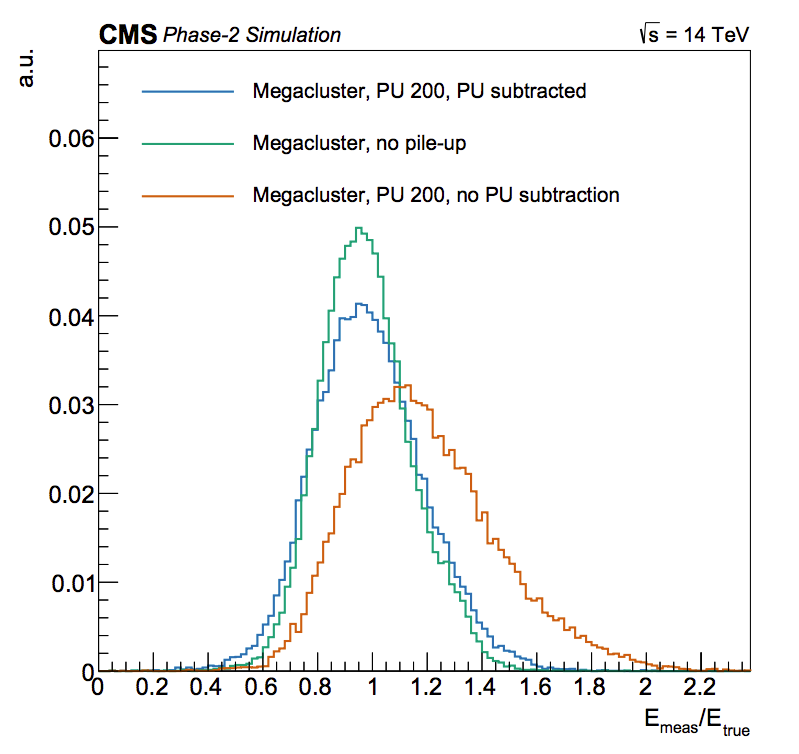
\includegraphics[width=0.6\textwidth]{Figures/HGCAL/SingleMegacluster.png}
\caption{The energy resolution for single $p_{T} =$ 25 GeV pions reconstructed using the megaclustering algorithm, before and after pileup subtraction. Taken from \cite{HGCAL}.}
\label{fig:SingleMegacluster}
\end{centering}
\end{figure}

The HGCAL's intrinsic performance measuring the energy of electromagnetic showers is modelled using a dedicated simulation with pileup corresponding to an average of 200 interactions per bunch crossing. 
Energy deposits in a radius of \SI{26}{mm} around a single unconverted photon are summed to estimate the energy resolution, which is shown in Figure \ref{fig:PhotonReso}.
The left plot shows that the resolution is approximately constant as a function of $\eta$, and robust against pileup, with only a very small degradation in resolution between PU0 and PU200.
This intrinsic performance is further demonstrated by using this method to reconstruct unconverted photon pairs from simulated \Hgg decays, 
where both photons are contained within the fiducial region of the HGCAL and the vertex location is assumed to be known exactly. 
The resulting diphoton mass distribution is shown in Figure \ref{fig:PhotonReso}, with resolution of around 1.8 GeV.
This value is comparable to the expected resolution of the upgraded CMS barrel calorimeter, representing a substantial improvement relative to Run 2. 

The HGCAL provides more detailed shower information than existing CMS detectors, 
and it is envisaged that eventually a sophisticated four-dimensional particle flow approach will be used to incorporate as much of this information as possible. 
In the meantime, more straightforward approaches to reconstruction have been developed, 
in order to understand which approaches are feasible and to produce object and physics-level results that demonstrate the potential of the detector. 

Furthermore, no use is yet made of the intrinsic timing capabilities of the silicon sensors, which will be invaluable in reducing the amount of out-of-time pileup at the HL-LHC. 
The current method begins by clustering hits in each two-dimensional (2D) layer independently, using an imaging algorithm \cite{ClusteringAlgo}.
These 2D or layer clusters are then associated together in depth to form so-called multiclusters. 
This step is performed by starting with the highest energy 2D cluster, then adding any other clusters sufficiently close in $\eta-\phi$ space. 
It is anticipated that this two-step process could be improved by performing 3D clustering directly, but this remains to be studied in detail. 

Electromagnetic objects are then formed using a superclustering procedure very similar to the one utilised in Run 2, 
collecting together showers which have been spread out in the $\phi$ by the magnetic field. 
Electrons defined in this way are used to test the ability of the HGCAL to discriminate between signal and background processes. 
Lateral and longitudinal shower shape variables, along with tracking information, are used as inputs to a Boosted Decision Tree (BDT) classifier. 
For a 95\% signal efficiency, the background efficiency is 1\% for electrons with $\pt > 20$ GeV, comparable to the Run 2 value. 
An improvement in performance is seen when both lateral and longitudinal shape variables are added to a classifier using track-only information. 
Additional studies applying the anti-$k_T$ algorithm directly on calorimeter hits to form jets have also been performed.
Constructing a pileup jet identification using just two variables, one each related to the lateral and longitudinal jet shape, 
was shown to be permit an acceptable L1 trigger rate of 10kHz for a signal efficiency of 80\%. 

Single hadrons were reconstructed using a so-called megaclustering procedure, where multiclusters within a truncated cone are combined to form the object. 
For these more dispersed hadronic showers, the resolution substantially improves once the contribution of pileup is subtracted.
The PU subtraction was implemented by removing the total energy of a similar cone randomly rotated in $\phi$. 
The energy resolution for a single pion with $\pt = 25$ GeV before and after the subtraction is shown in Figure \ref{fig:SingleMegacluster}. 
The megaclustering algorithm is shown to yield adequate energy resolution of around 20\%. 
It is also robust against pileup, showing a modest worsening between PU0 and PU200 that decreases quickly as a function of \pt.

\subsection{Physics performance}

\begin{figure}[h!]
\begin{centering}
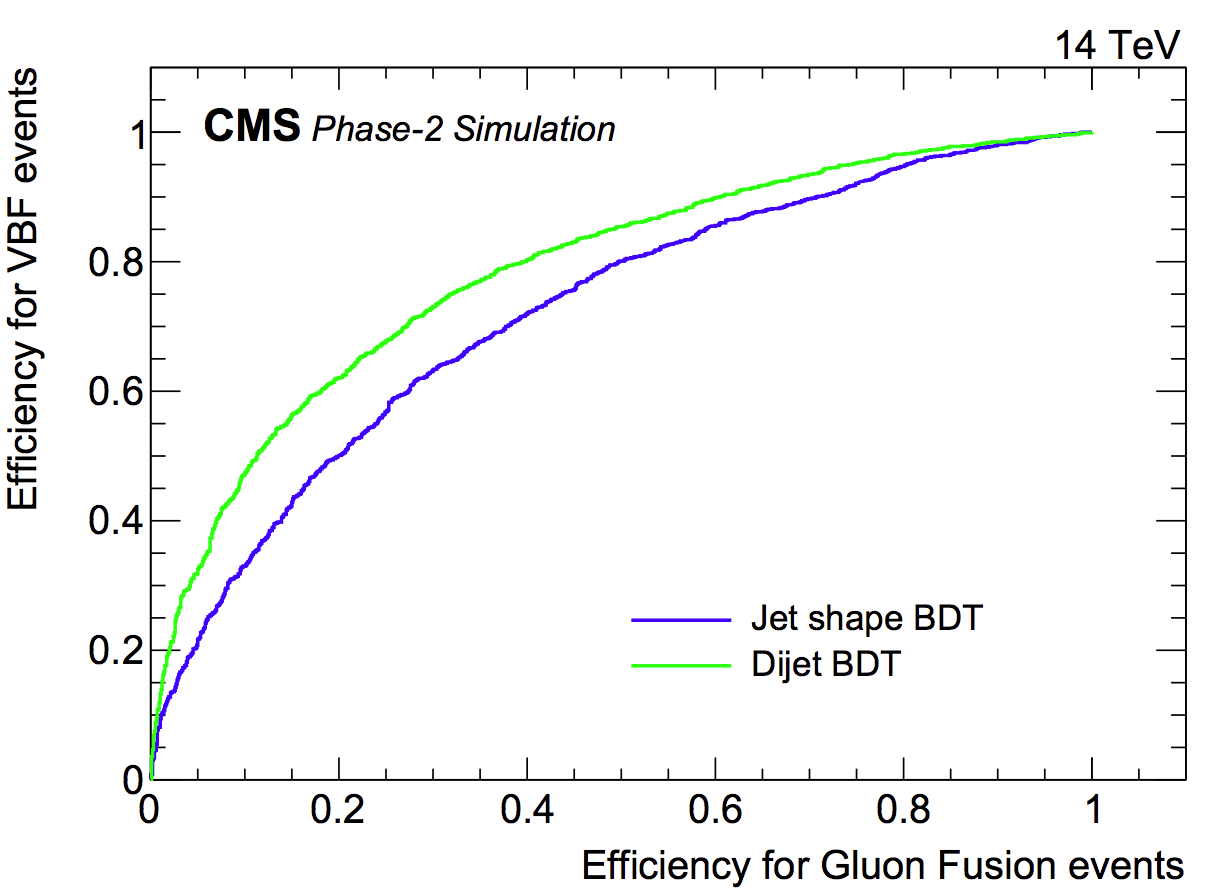
\includegraphics[width=0.65\textwidth]{Figures/HGCAL/VBFvsGGH.png}
\caption{The selection efficiency for VBF and ggH events for two different BDT setups. Taken from \cite{HGCAL}.}
\label{fig:VBFvsGGH}
\end{centering}
\end{figure}

One of the main benefits of the HGCAL upgrade will be the ability to separate real VBF jets from those originating from gluon emission.
This is illustrated in a study of the two production modes in the \Hgg decay channel.
Two Boosted Decision Tree (BDT) classifiers are constructed, one using only jet shape variables and another including further jet and photon kinematic variables. 
The latter is very similar to one used in the existing Run 2 analysis.
The performance of the jet shape only BDT, measured using the area under the ROC curve shown in Figure \ref{fig:VBFvsGGH}, is 0.71. 
This improves to 0.79 with the full kinematic information included, and is even higher than the Run 2 performance of 0.75. 
With \SI{3000}{\fbinv} of data, a suitably chosen cut on this BDT would yield 750 signal events, with 75\% VBF purity, for a background of 678 events per GeV, comparable to the Run 2 values. 

\subsection{Beam tests}

\begin{figure}
\centering
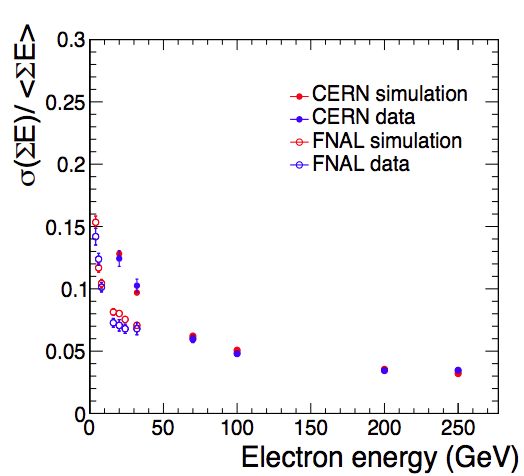
\includegraphics[width=.5\textwidth]{Figures/HGCAL/BeamTestElectronReso.png}
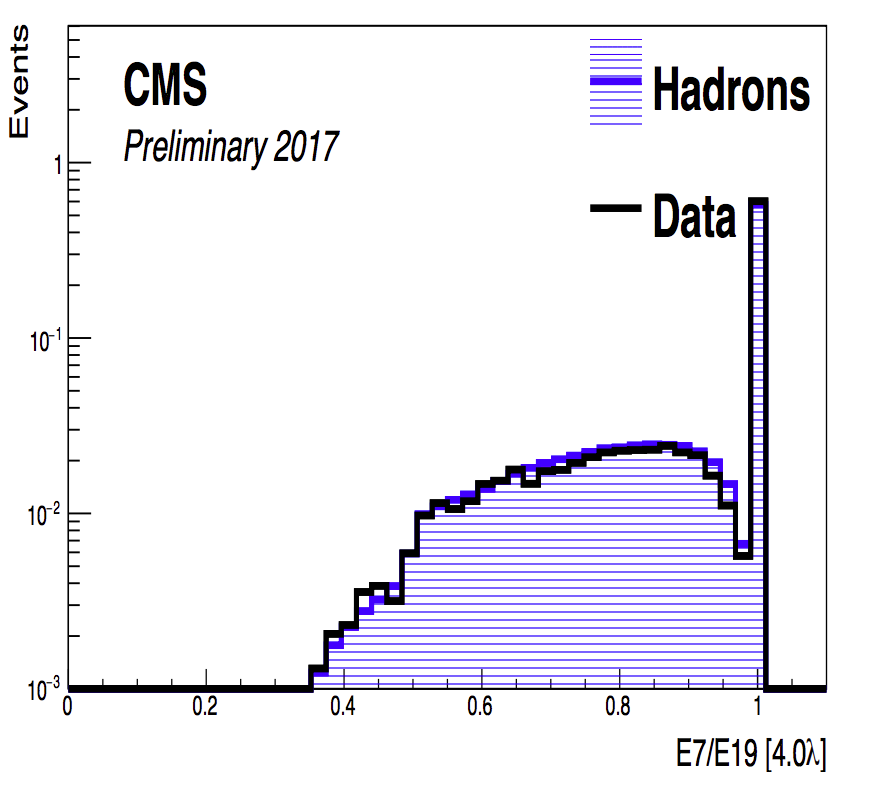
\includegraphics[width=.49\textwidth]{Figures/HGCAL/BeamTestHadronReso.png}
\caption{
Left: electron energy distribution for both data and Monte Carlo simulation.
Right: Transverse shower shape distribution in the CE-H. 
}
\label{fig:BeamTest}
\end{figure}

To validate the design of the HGCAL and ensure its behaviour is well-modelled by simulation, beam tests have been conducted at both CERN and Fermilab sites in 2016 and 2017. 
Prototype silicon modules representative of those in both the CE-E and CE-H were built, with plastic scintillator tiles modified from an existing detector developed by the CALICE collaboration.
Comparisons of the measured electron energy resolution and hadronic shower shape to simulation are shown in Figure \ref{fig:BeamTest}.
These prototypes were not the full design thickness, so the performance is not representative of the final detector.
However the results constitute the first demonstration that the HGCAL behaves as predicted by simulation; observed distributions match those predicted by simulation to within 5\%. 
Furthermore, the tests confirm the intrinsic timing capabilities of the silicon sensors, with timing resolution measured to be less than 30ps.
The timing performance of the silicon was also confirmed to be a function of S/N only, and not degrade with increasing radiation exposure. 

The HGCAL project is designed to replace the existing CMS endcap calorimeters and withstand the harsh HL-LHC conditions for its full lifetime.
Offering unprecedented granularity in lateral and longitudinal directions, it is expected to provide detailed three-dimensional images of showers in addition to precision timing information from the silicon sensors. 
This will allow for powerful pileup rejection, sophisticated pattern recognition within CMS particle flow, and precise energy measurements. 
The recent technical design report showcased the potential of the detector, and between now and installation in 2026 much work remains to be done to overcome the many technical challenges ahead.
